\documentclass[11pt]{article}

\usepackage[margin=1.0in]{geometry}
\usepackage{natbib}
\usepackage{changepage}
\usepackage{rotating}
\usepackage{graphicx,amsmath,amssymb,amsfonts}
\sloppy

\pdfminorversion 4


\bibpunct[,]{(}{)}{;}{a}{}{,}


\begin{document}

\title{\textbf{Supplementary Material for ``Limited utility of residue masking for positive-selection inference"}}
\author{Stephanie J. Spielman$^{1*}$ and Eric T. Dawson$^{1}$ and Claus O. Wilke$^{1}$}
\date{}
\maketitle
\noindent $^1$Department of Integrative Biology, Center for Computational Biology and Bioinformatics, and Institute of Cellular and Molecular Biology.
\\ The University of Texas at Austin, Austin, TX 78712, USA.\\

\bigskip
\noindent
$^*$Corresponding author\\
$\phantom{^*}$Email: stephanie.spielman@utexas.edu\\

\bigskip
\tableofcontents

\newpage 

\section{Materials and Methods}

\subsection*{Guidance Software Reimplementation and Scoring Algorithms}
Our reimplemented Guidance is written in Python and C++ and is described in detail in SI. Following the algorithm set forth in Penn et al. \citep{Penn2010}, we first create a reference multiple sequence alignment (MSA) using a user-specified progressive MSA software, with choices of Clustalw \citep{Thompson1994}, MUSCLE \citep{Edgar2004}, or MAFFT \citep{Katoh2002, Katoh2005}. We then generate $N$ (where $N=100$, by default) bootstrapped MSA replicates, each of which is used to create a bootstrapped tree in FastTree2 \citep{Price2010}. We then use these $N$ trees as guide trees to create $N$ new perturbed MSAs, which we subsequently compare to the reference MSA to generate a confidence score for each residue. Users can specify options for their aligner and phylogeny reconstruction method as desired.

Before calculating confidence scores, a phylogeny is built from the reference MSA. Our program includes functionality to build this phylogeny using either FastTree2 \citep{Price2010} or RAxML \citep{Stamatakis2006}. Two types of phylogenetic weights can be calculated from this tree. The first uses the software package BranchManager \citep{Stone2007} to calculate a weight for each taxon in the phylogeny representing that taxon's contribution to the phylogeny as a whole. We call this method ``BMweights." The second method calculates patristic distances (sum of branch lengths) between each taxon in the phylogeny using the python package DendroPy \citep{Sukumaran2010}. We call this method ``PDweights."

We calculate positional confidence scores for each of the $N$ bootstrap MSAs as follows. A raw score, $S_{ij}$, for a given residue in row $i$, column $j$ of the reference MSA is calculated as \begin{equation} S_{ij} = \sum\limits_{k \in R_\text{ng}^{(j)}} I_{ik}^{(j)} s_{ik}   ,\end{equation} where $R_\text{ng}^{(j)}$ represents the set of rows in column $j$ which are not gaps. We calculate $s_{ik}$ according to the given scoring algorithm:
\begin{equation}
s_{ik}} = \left\{ \begin{array}{rl}

              1                         &\mbox{if Guidance} \\
              w_iw_k              &\mbox{if BMweights} \\
              d_p(i,k)              &\mbox{if PDweights} \\
                     \end{array} \right.,
\end{equation} where $w_i$ is the phylogenetic weight of the taxon at row $i$, as calculated by BranchManager, and $d_p(i, k)$ is the patristic distance between the taxa at rows $i$ and $k$. 
The indicator function 
\begin{equation}I_{ik}^{(j)} = \left\{ \begin{array}{rl}

              1                         &\mbox{if reference MSA residue pair $(i, k)^{(j)}$ is present in bootstrap MSA} \\
              0            &\mbox{if reference MSA residue pair $(i, k)^{(j)}$ is absent in bootstrap MSA} \\
                     \end{array} \right. 
\end{equation}
serves to compare the bootstrap- and reference-MSA residue pairings.


We then sum positional scores $S_{ij}$ determined from each bootstrap replicate $n$. We normalize these scores across bootstrap replicates to yield a final score $\widetilde{S}_{ij}$ for each residue in the reference MSA. We use two different normalization schemes: original Guidance (defined in \citet{Penn2010}) and a novel gap-penalization scheme. These normalization schemes are given by \begin{equation}
\widetilde{S}_{ij}  = \sum_n S_{ij}(n) \bigg{/} \left\{ \begin{array}{rl}

              \sum\limits_n \sum\limits_{k \in R_\text{ng}^{(j)}} s_{ik}(n)     &\mbox{if original Guidance} \\
              \sum\limits_n \sum\limits_{k \in R_\text{all}^{(j)}} s_{ik}(n)     &\mbox{if gap-penalization} \\      
        \end{array} \right.,
\end{equation} 
where $R_\text{all}^{(j)}$ represents all rows in column $j$, including gaps, the sums over $n$ run over all $N$ replicates, and $S_{ij}(n)$ and $s_{ik}(n)$ each represent those respective quantities for bootstrap replicate $n$. By considering all rows instead of just rows that are not gaps, the gap-penalization scheme will naturally assign lower scores to highly gapped columns. We refer to the algorithms normalized by the original Guidance scheme as Guidance, BMweights, and PDweights. When normalized with the gap-penalization scheme, we refer to them, respectively, as GuidanceP, BMweightsP, and PDweightsP. Note that scores calculated using the Guidance algorithm with the original normalization scheme are equivalent to those originally derived by \citet{Penn2010}. 



\subsection*{Sequence Simulation}
Coding sequences were simulated using Indelible \citep{Fletcher2009}. To ensure that our simulations reflected realistic protein sequences, we simulated sequences according to two distinct sets of evolutionary parameters. The first selective profile was derived from H1N1 hemagluttinin (HA) influenza protein, and the second selective profile was derived from HIV-1 envelope protein GP41, which contains only the cytosolic and tail regions. 

To derive parameters for the HA selective profile, we aligned 1038 HA protein sequences collected from the Influenza Research Database (http://www.fludb.org) with MAFFT, specifying the ``--auto" flag, \citep{Katoh2002,Katoh2005} and then back-translated to a codon MSA using the original nucleotide sequence data. We generated a phylogeny from this codon MSA in RAxML \citep{Stamatakis2006} using the GTRGAMMA model. Using the codon MSA and phylogeny, we inferred evolutionary parameters as described \citep{Spielman2013}. We used a REL (random effects likelihood) method \citep{NielsenYang1998} using the HyPhy software \citep{Pond2005}, with five $dN/dS$ rate categories as free parameters under the GY94 evolutionary model \citep{GoldmanYang1994}. We employed a Bayes Empirical Bayes approach \citep{Yang2000} to obtain infer $dN/dS$ values at each site, which we used to assess a complete distribution of site rates. The resulting $dN/dS$ had a mean of 0.37. We binned these rates into 50 equally spaced categories for specification in Indelible, which required a discrete distribution of $dN/dS$ values. Again according to parameters derived from the HA analysis, we fixed $\kappa$, the transition-to-transversion ratio, at 5.3 and set state codon frequencies equal to those directly calculated from the HA MSA. 

To derive parameters for the GP41 selective profile, we aligned 2192 sequences from the LANL database (http://HIV.lanl.gov), again with MAFFT. We generated an amino-acid phylogeny from this MSA using FastTree2 under the WAG model. We subsequently inferred a $dN/dS$ distribution from this data in FUBAR. Note that we only used those $dN/dS$ values which were below 6, as FUBAR's approximate approach yielded estimates well over 1000 when $dS$ values were small. Again, we binned the resulting $dN/dS$ distribution into equally spaced categories for specification in Indelible. The resulting $dN/dS$ distribution had a mean of 0.89. We inferred a value for $\kappa$ by selecting from this large dataset a random set of 150 sequences, which we aligned with linsi \citep{Katoh2002,Katoh2005} and inferred a phylogeny using FastTree2 \citep{Price2010}, specifying the options ``-wag -fastest." We then inferred $\kappa$, which was calculated as 3.36, using the GY94 model in HyPhy. For all simulations under the GP41 selective profile, we fixed $\kappa$ at 3.36 and set state codon frequencies equal to those directly calculated from the GP41 MSA. 

We simulated 100 alignments across four different real gene trees each, for both selective profiles, yielding a total of 800 simulated MSAs. Phylogenies used included an 11-taxon tree of the mammalian olfactory receptor OR5AP2 \citep{Spielman2013}, a 26-taxon tree of mammalian rhodopsin sequences \citep{Spielman2013}, a 60-sequence tree of phosphoribulokinase (PRK) genes from photosynthetic eukaryotes \citep{Yang2011}, and a 158-taxon multilocus tree of flatfish sequences \citep{Betancur2013}. The latter two phylogenies were obtained from TreeBASE (http://treebase.org). We set all insertion-deletion (indel) rates at 0.05, motivated by studies demonstrating that indel events occur at a rate 5\% of the substitution rate in mammalian genomes \citep{Cooper2004}, and we set all average sequence lengths to 400 codons.

\subsection*{MSA Construction and Positive-Selection Inference}

We build all MSAs using MAFFT L-INS-I (linsi) \citep{Katoh2002,Katoh2005} within the context of our Guidance reimplementation. Phylogenies used to calculate phylogenetic weights for the BMweights and PDweights algorithms were constructed in RAxML, specifying ``PROTGAMMAWAG" as the model of sequence evolution \citep{Stamatakis2006}. In addition to an unfiltered MSA, we generated six filtered MSAs (one for each filtering algorithm and each normalization scheme), masking residues with scores $\leq0.5$ with ``?". To investigate potential biases introduced by the scoring threshold, we also masked residues below the scoring cutoffs of 0.3, 0.7, and 0.9 for MSAs constructed with the Guidance and GuidanceP filters. Only MSAs simulated according to HA parameters were included for this analysis.

We inferred positive selection using both the PAML M8 model \citep{Yang2007} and FUBAR \citep{Murrell2013}, which is implemented in the HyPhy \citep{Pond2005} software package. For inference with PAML, we specified the $F3\times4$ codon frequency model and ``cleandata = 0" in the control file. For FUBAR inference, we used mostly default parameters, except when specifying grid dimensionality. As neither Indelible nor PAML simulates sequences without $dS$ variation, we specified that FUBAR only consider $dN$ variation, in order to make results from FUBAR and PAML fully comparable. We additionally specified 100 grid points to account for the reduced grid dimensionality caused by ignoring $dS$ variation. Phylogenies specified for positive-selection inference were those constructed during the Guidance MSA procedure when deriving phylogenetic weights. All filtered MSAs derived from a unfiltered MSA were processed with identical phylogenies to avoid potentially confounding effects of different tree topologies. Note that while we employed FUBAR to assess positive selection for all simulation sets, we did not use PAML to infer positive selection for the largest set (158 sequences).

We then compared resulting positive-selection inferences for each MSA to its respective true MSA's $dN/dS$ values, given by Indelible during simulation, to assess performance accuracy. As residues may have been differently aligned relative to the true simulated MSA, we constructed a map from each unfiltered MSA to its respective true MSA. For this map, we selected the sequence in the unfiltered MSA with the fewest number of gaps and mapped its non-gap sites to the corresponding residue position in the true MSA. This strategy ensured that the most sites possible were included when calculating true positive rates. Importantly, all filtered variants of a given unfiltered MSA used the same map to the true MSA. We considered sites positively selected if the posterior probability of $(dN/dS>1)$ was $\geq0.9$.

All statistics were conducted using Python and R. Linear modeling was conducted using the R package lme4 \citep{Bates2012}. We inferred effect magnitudes and significance, which we corrected for multiple testing,g using the R multcomp package's glht() function with default settings \citep{Hothorn2008}. All code used in this study is available at https://github.com/clauswilke/alignment\underline{\hspace*{0.2cm}}filtering.

\section*{Analysis of MSA Filtering Threshold}
When filtering MSAs with Guidance-based methods, one must select a specific score cutoff below which to mask residues. We chose to filter all residues with scores less than 0.5, as previously done by \citet{Jordan2012}. However, \citet{Privman2012} filtered all sites which scored below a threshold of 0.9. Therefore, it was possible that selecting a different threshold would have yielded different results, so we analyzed how changing this threshold might impact our findings. For this analysis, we considered only the Guidance and GuidanceP scoring schemes for the HA selective profile. Using the same position confidence scores previously generated, we masked all alignments at the additional cutoffs of 0.3, 0.7, and 0.9 and inferred positive selection with FUBAR and PAML as described.

We fit mixed-effects linear models for each simulation set, with TPR as the response, masking cutoff as a fixed effect, and simulation count as the random effect, for Guidance and GuidanceP results each. In general, the threshold of 0.3, 0.5, and 0.7 performed statistically indistinguishably. The single exception to this finding occurred for the 60-sequence simulation set, as inferred with FUBAR, for which the cutoffs of 0.3 and 0.5 each performed marginally better than did the 0.7 cutoff ($P < 0.01$ and $P < 0.05$, respectively). However, as shown in Table S1, the cutoff of 0.9 tended to yield worse performances than did the 0.5 threshold. It is, however, important to note that PAML was generally more robust to changes in masking threshold than was FUBAR, and that GuidanceP was influenced more by changing the masking threshold than was Guidance. Likely the latter observation resulted from the fact that the gap-penalization algorithms mask far more sites than do algorithms which use the original normalization scheme, ultimately resulting in an excessive amount of information removed at a 0.9 masking threshold.

Therefore, we do not expect that our results were biased by our selection of a 0.5 masking threshold. Alternatively, using a stringent 0.9 cutoff likely would have excessively sacrificed power for positive-selection inference in several cases. 

\bigskip
\begin{table}[htbp]
\begin{adjustwidth}{-1.5cm}{}
\noindent \textbf{Table S1.} Effect of masking cutoff on mean TPR of positive-selection inference for filtered MSAs.
\begin{tabular}{l l c c c c c c c}
\hline\noalign{\smallskip}
& & \multicolumn{3}{c}{Guidance} & & \multicolumn{3}{c}{GuidanceP}   \\
\cline{3-5} \cline{7-9}\noalign{\smallskip}
\multicolumn{1}{c}{Taxa} & \multicolumn{1}{c}{Method} & \multicolumn{1}{c}{0.5 TPR} & \multicolumn{1}{c}{0.9 TPR} & \multicolumn{1}{c}{Percent TPR Change} & & \multicolumn{1}{c}{0.5 TPR} & \multicolumn{1}{c}{0.9 TPR} & \multicolumn{1}{c}{Percent TPR Change}  \\
\hline\noalign{\smallskip}
11  &  FUBAR  &  0.085  &  0.082  &  \textbf{-4.22\%$^{\ast}}$  & &  0.085  &  0.079  &  \textbf{-6.60\%$^{\ast\ast}$}  \\
  &  PAML  &  0.082  &  0.079  &  -2.59\% & &  0.081  &  0.074  &  \textbf{-8.38\%$^{\ast\ast}$}   \\
\hline
26  &  FUBAR  &  0.229  &  0.227  &  -0.87\% & &  0.226  &  0.215  &  \textbf{-5.21\%$^{\ast\ast\ast}$}  \\
  &  PAML  &  0.178  &  0.179  &  0.67\% & &  0.183  &  0.175  &  \textbf{-4.33\%$^{\ast\ast}$}  \\
\hline
60  &  FUBAR  &  0.479  &  0.458  &  \textbf{-4.43$^{\ast\ast\ast}$} & &  0.464  &  0.332  &  \textbf{-28.5\%$^{\ast\ast}$}  \\
  &  PAML  &  0.342  &  0.327  &  -4.19\%  & &  0.337  &  0.256  &  \textbf{-24.1\%$^{\ast\ast}$}  \\
\hline
158  &  FUBAR  &  0.467  &  0.463  &  -0.73\%  & & 0.468  &  0.452  &  \textbf{-3.44\%$^{\ast\ast\ast}$}  \\
\hline
\end{tabular}
\newline
\textsc{note.}--- Significance levels: $^{\ast\ast\ast} P < 10^{-4}$; $^{\ast\ast} P < 10^{-3}$; $^{\ast} P < 10^{-2}$. 
0.5 TPR: average TPR for MSAs masked at a cutoff of 0.5; 0.9 TPR: average TPR for MSAs masked at a cutoff of 0.9; Percent TPR Decrease: average percent decrease in TPR recovered between MSAs masked at cutoffs of 0.5 and 0.9. Linear models were conducted with the lme4 package in R \citep{Bates2012}. All significance levels were corrected for multiple comparisons using the multcomp package in R \citep{Hothorn2008}.
\end{adjustwidth}
\end{table}




\newpage
\section{Supplementary Figures}


\centerline{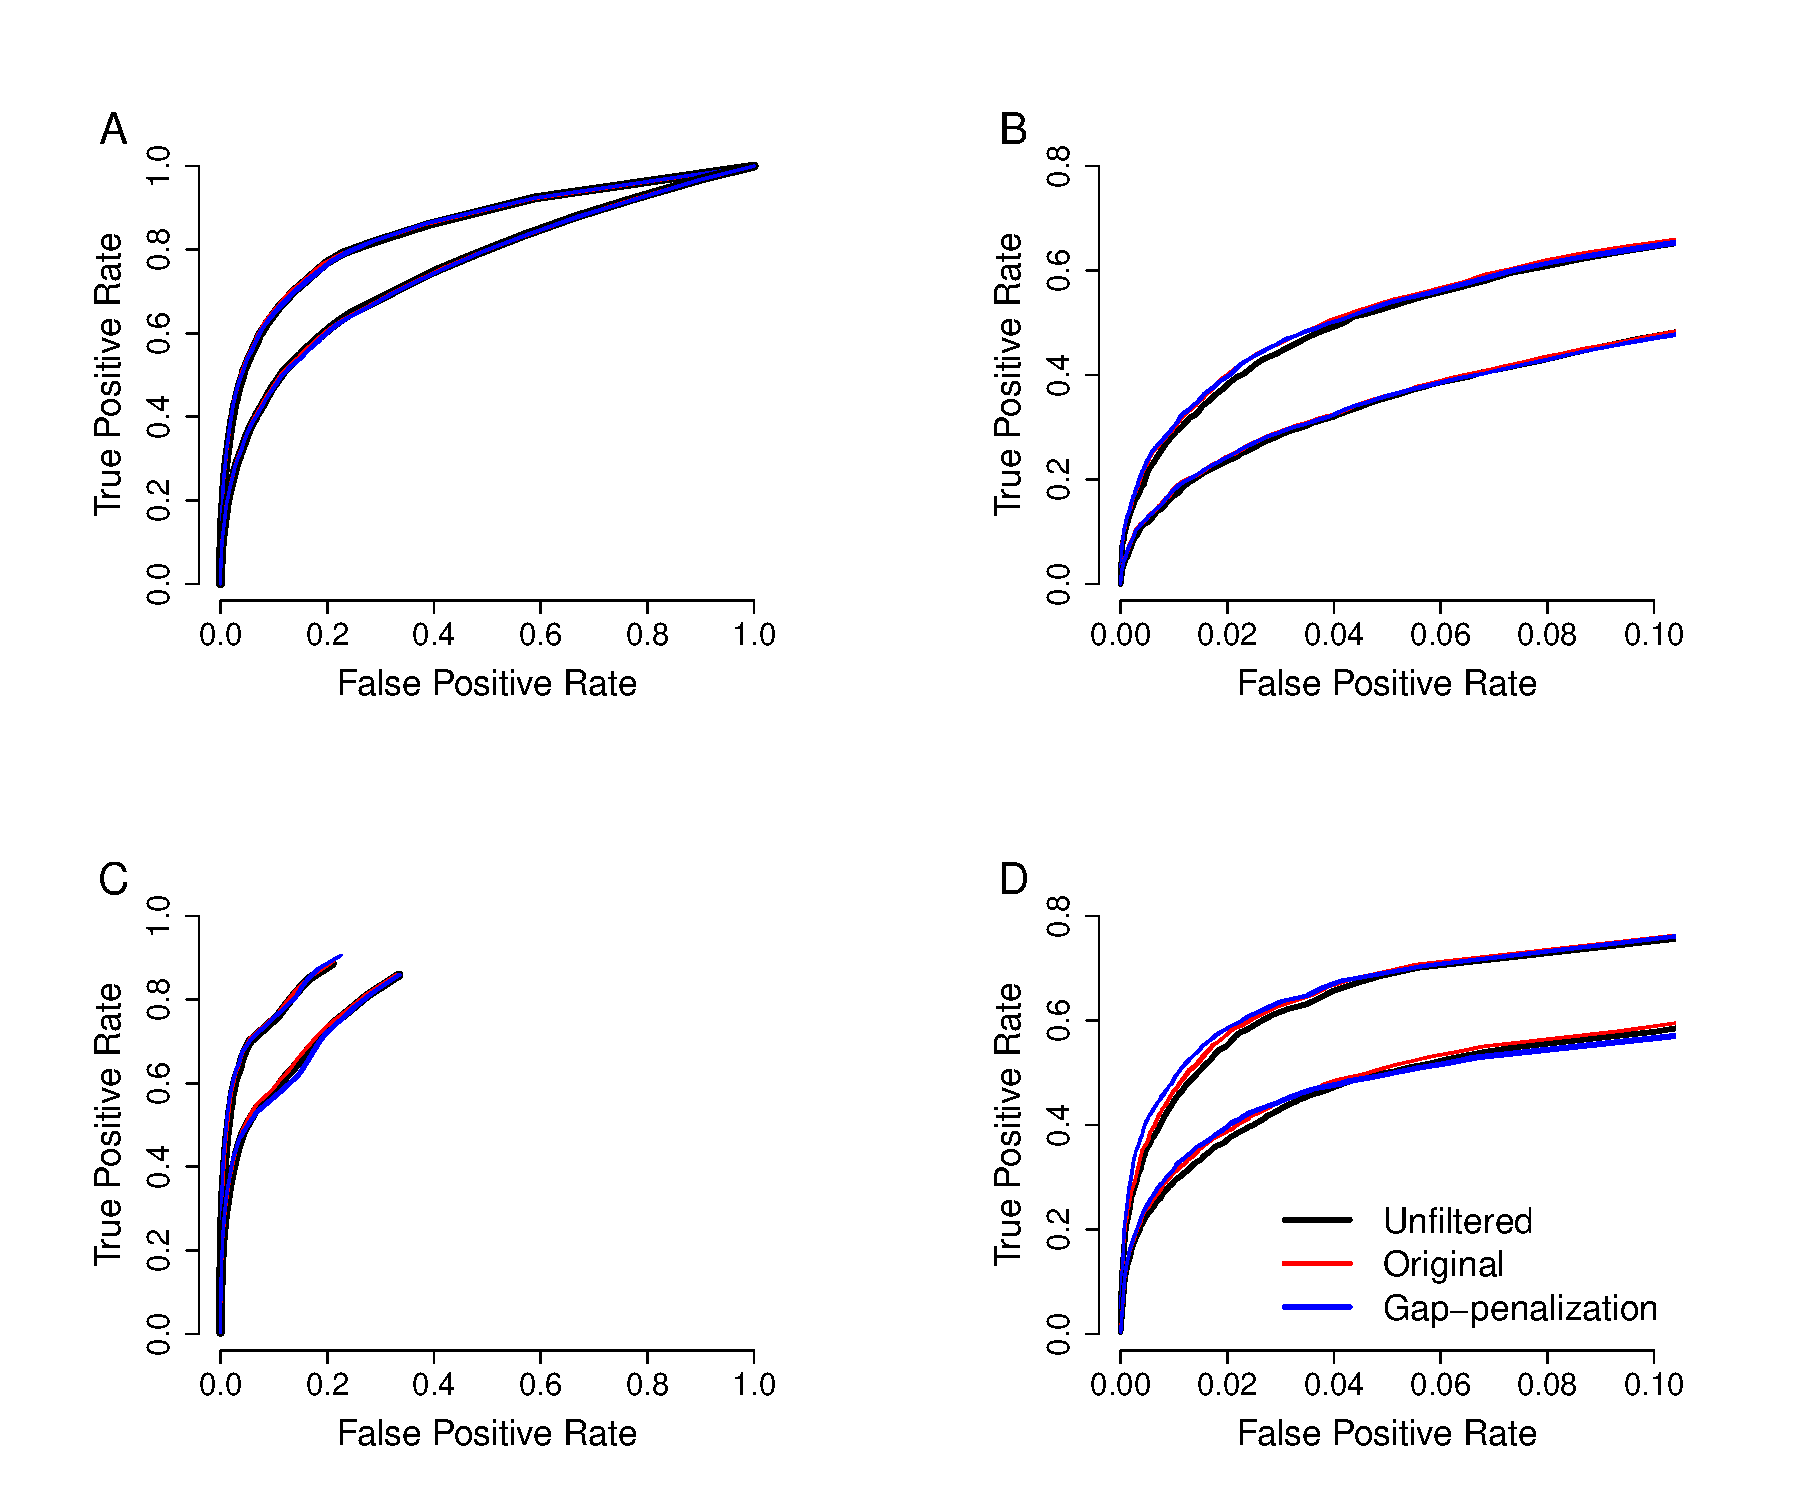
\includegraphics[width=6.5in]{Figures/ROC_SI_paml.pdf}}
\noindent \textbf{Figure S1.} ROC curves for positive-selection inference with PAML M8, averaged within each simulation set. For all panels, the top curve represents results from the HA selective profile, and the bottom curve represents results from the GP41 selective profile. The left-hand panels display the entire ROC curves, while the right-hand panels display only the region of the curves with relatively low FPRs. Note that, for the full ROC curves, methods only achieved FPR levels shown. A-B) ROC curves for the 11-sequence simulation sets. C-D) ROC curves for the 26-sequence simulation sets.

\newpage
\centerline{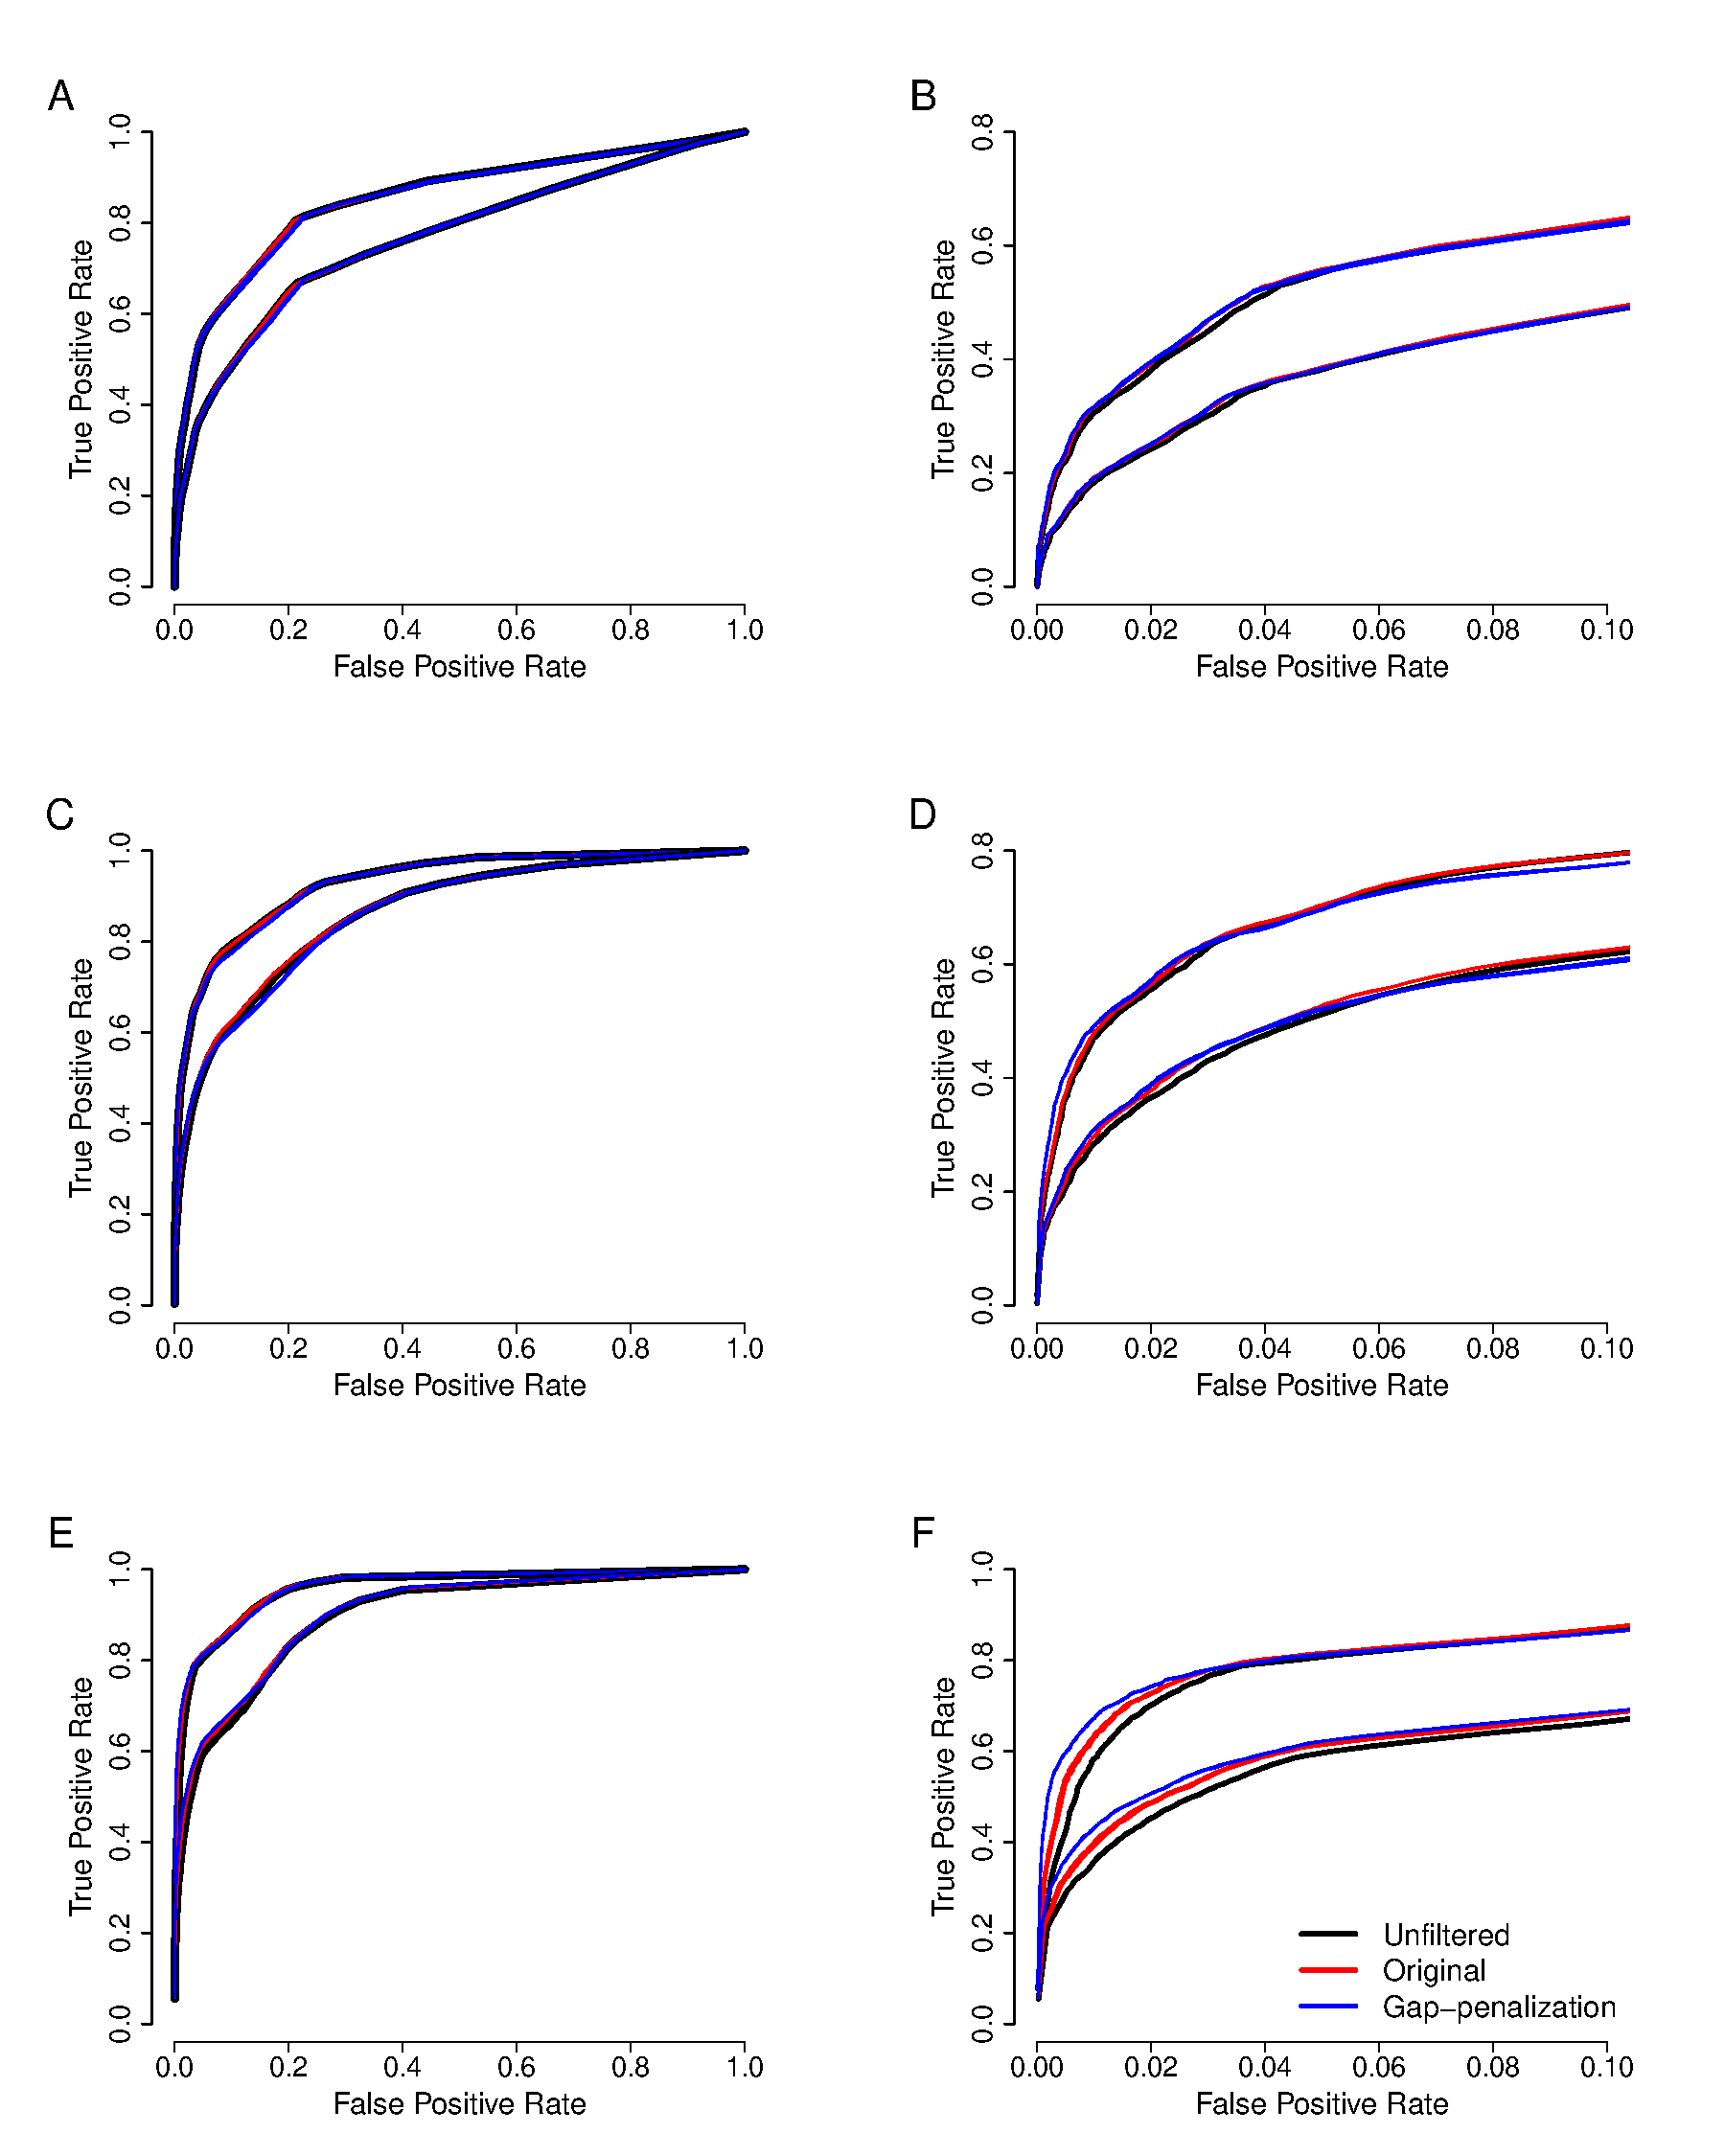
\includegraphics[width=6.25in]{Figures/ROC_SI_fubar.pdf}}
\noindent \textbf{Figure S2.} ROC curves for positive-selection inference with FUBAR, averaged within each simulation set. For all panels, the top curve represents results from the HA selective profile, and the bottom curve represents results from the GP41 selective profile. The left-hand panels display the entire ROC curves, while the right-hand panels display only the region of the curves with relatively low FPRs.  A-B) ROC curves for the 11-sequence simulation sets. C-D) ROC curves for the 26-sequence simulation sets. E-F) ROC curves for the 158-sequence simulation sets.

\newpage

\bibliographystyle{MBE}
\bibliography{citations}	




\end{document}